%\title{Building Perfect Brackets}

\documentclass[5p, preprint]{elsarticle}

\usepackage[cmex10]{amsmath}
\usepackage[parfill]{parskip}
\usepackage{url}
\usepackage{graphicx}
\usepackage{subfig}
\usepackage{caption}
\usepackage{hyperref}

% correct bad hyphenation here
\hyphenation{op-tical net-works semi-conduc-tor}

\begin{document}

\title{Building Perfect Tournament Brackets with Data Analytics}

\author[purdue_ChE]{Christopher D. Hagmann\corref{cor1}}
\ead{chagmann@purdue.edu}

\author[purdue_BME]{Nan Kong}
\ead{nkong@purdue.edu}

\cortext[cor1]{Corresponding author}


\address[purdue_ChE]{School of Chemical Engineering, Purdue University, 480 Stadium Mall Drive, West Lafayette, IN 47907, USA}
\address[purdue_BME]{Weldon School of Biomedical Engineering, Purdue University, West Lafayette, IN 47907, USA}


\begin{abstract}
The NCAA men's basketball tournament highlights data analytics to the everyday person as they look for help building their brackets. A k-Nearest Neighbors algorithm is proposed to compare new opponents to previously played teams. A distance between teams is calculated to determine the most similar teams and to weigh the value of each win or loss to the teams. The value of $k$ is determined from previous years and applied to 2014. Results are compared to other predictions for 2014.
\end{abstract}


% Note that keywords are not normally used for peerreview papers.
\begin{keyword}
k-Nearest Neighbors (kNN); March Madness; Tempo-free Statistics.
\end{keyword}


% The paper headers
\markboth{Working Paper}%
{Hagmann \MakeLowercase{\textit{et al.}}: Building Perfect Brackets}


\maketitle

\section{Introduction}

Every March in the United States, work productivity dramatically drops as everyone turns their attention to the National Collegiate Athletic Association (NCAA) Division 1 (D-I) men's basketball tournament, known colloquially as ``March Madness."  This single elimination, or knockout, tournament consists of 64 teams in four groups of 16, with each group being ranked (or ``seeded'') so that the highly favored teams do not have to compete until later in the tournament. A popular tradition that accompanies this event is tournament pools. In tournament pools, groups of people submit fill-in tournament brackets with their predictions of which team they think will win. As most pools have prizes for the winners, more and more people are turning to data analytics to help them build the perfect tournament bracket. 

This has never been as true as it was in 2014 when Warren Buffet announced a \$1,000,000,000 (USD) prize for anyone who correctly predicted all 63 games' outcomes. Figure \ref{pic:distro} shows the distribution of correctly predicted games of all 9,223,372,036,854,775,808 possible brackets, assuming that each bracket is just as likely to occur as any other bracket. Figure \ref{pic:distro} also shows the real-life distributions based on the 2013 and 2014 ESPN Tournament Challenges. In this paper, a k-Nearest Neighbors algorithm is developed to attempt to better predict the perfect bracket.

\begin{figure*}[!t]
\centering
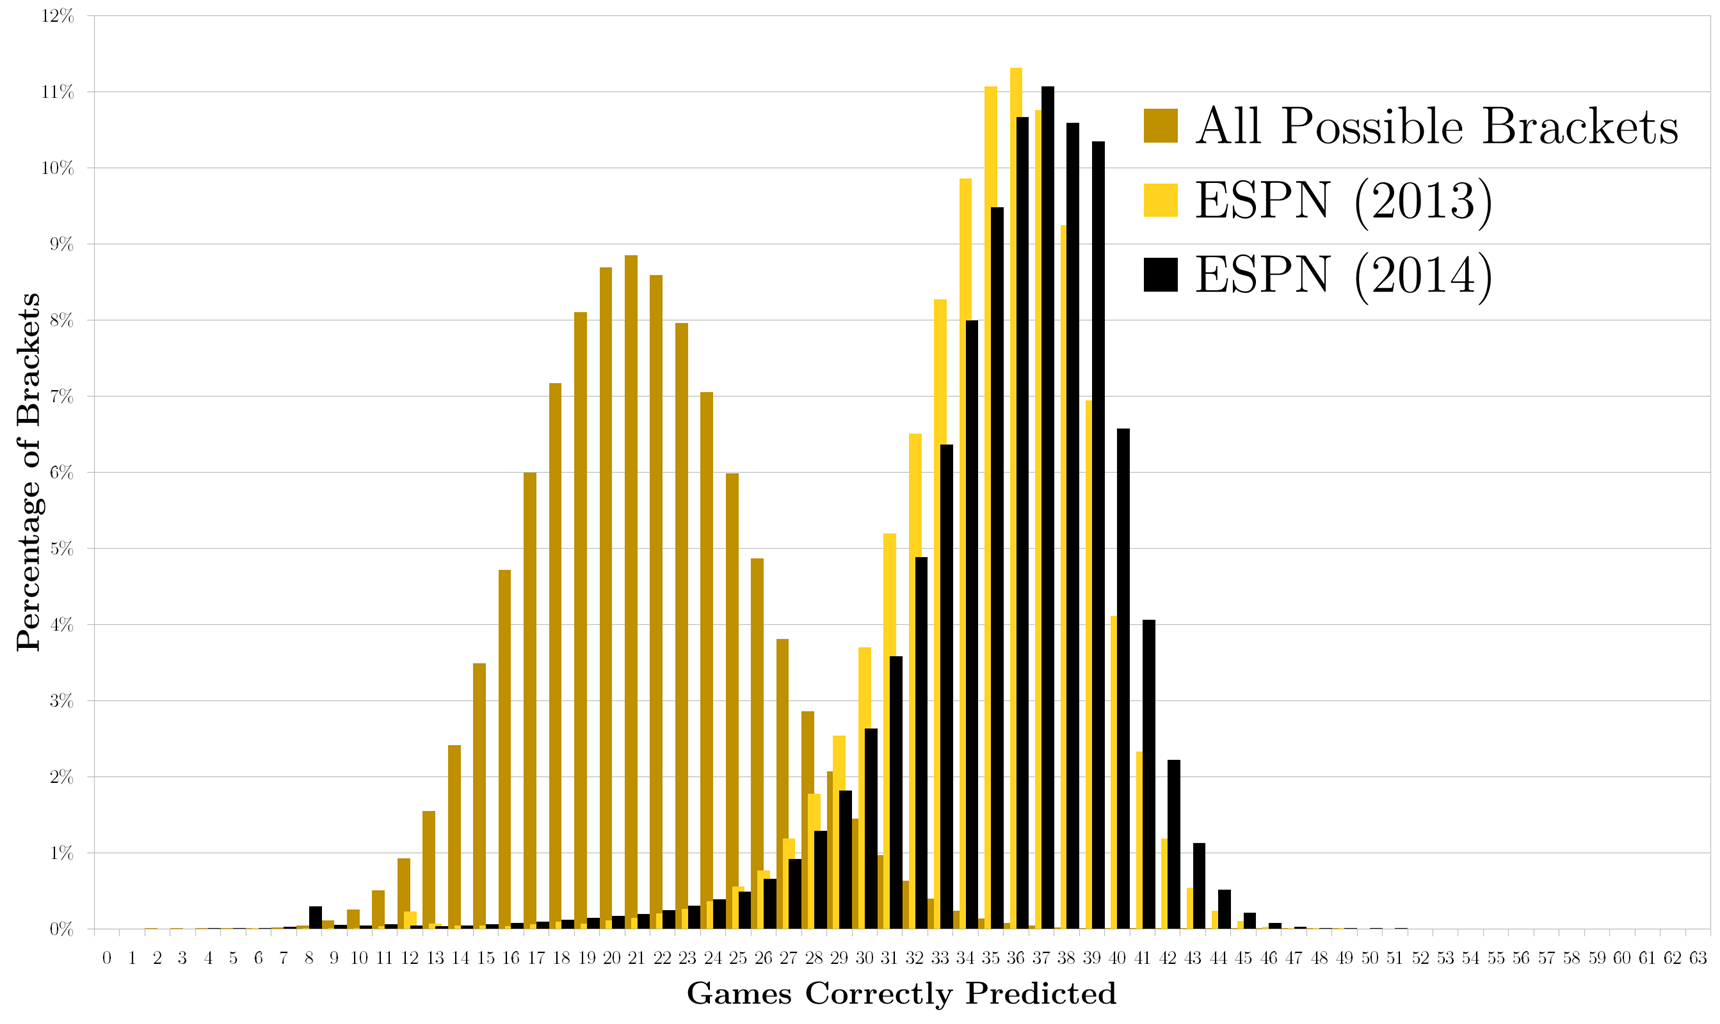
\includegraphics[width=6.5in]{distro2.png}
\caption{Distribution of the number of games correctly picked for all possible brackets along with the distributions of the 2013 and 2014 ESPN Tournament Challenges}
\label{pic:distro}
\end{figure*}

\vspace*{-.1in}

\subsection*{Tempo-Free Statistics}

Traditionally in basketball, team and player statistics are averaged on a ``per-game" (PG) basis. As such, when looking at a stats page on the NCAA D-1 men's basketball website, one will find the abbreviations PPG (points per game),  OPP PPG, (opponent's points per game), APG (assists per game), and RPG (rebounds per game).  In recent years, however, there has been a shift by some away from these statistics in exchange for statistics that are independent of a team's tempos. 

The tempo of a basketball team is defined by the number of possessions a team has in a game. In NCAA D-1 men's basketball, each team has 35 seconds to shoot the ball and at least hit the rim; otherwise, the ball is turned over to the other team.  There are some teams that will pass the ball frequently looking for the best open shot and use nearly all of this time, but there are others that try to make the first available shot they have. As such, the number of possessions a team has in a single 40-minute game can vary dramatically. 

There are many arguments for tempo-free statistic. First, basketball can be viewed as a turn-based game where every possession ends with points, a missed shot, or a turnover before possession is transferred to the other team. Consequently, the offense would like to convert possessions into as many points as possible while the defense would like to prevent the other team from doing so. Second, 40 minutes is not necessarily long enough to collect an adequate sample of possessions over which to average. Third,  the number of possessions in the game will differ. Therefore,  it is easier to compare teams on the per possession basis, or in other words, to use tempo-free statistics.   

For example, suppose Team A and Team B are going to play each other. Looking over the team statistices both teams average 80 points per game. They seem like a very even match; however, their tempos are 60 and 80 possessions per game, respectively. This means that Team A is averaging 4 points every 3 possessions while Team B is only averaging 4 points every 4 possessions. When teams play each other they will have nearly the same amount of possessions, save for who starts and ends with the ball. As such, it is easy to see that if the team's average points per possession hold, that Team A will beat Team B as it is more effective at converting possessions to points than Team B.

This idea of making statistics that are independent of a team's tempo, or tempo-free statistics, has been championed by analysts like Ken Pomeroy, who runs a site that provides tabulated tempo-free statistics (\href{kenpom.com}{kenpom.com}). It is important to note that all of these statistics are defined as some sort of estimate against an average D-I team. In other words, assuming a D-I team  throughout the course of the season has faced a good sample of D-I opponents, then their per-possession statistics are a good approximation for how they would do against the average D-I team. 

For example, the adjusted offensive efficiency($AdjOE$) is an estimate of the number of points scored a team would have against the average D-I defense per 100 possessions. The adjusted defensive efficiency($AdjDE$) is an estimate of the number of points allowed by a team against the average D-I offense per 100 possessions. 

Finally, the Pythagorean expectation($Pyth$) combines the adjusted offensive and defensive efficiencies for a D-I team. It is considered an estimate of the team's expected winning percentage against average D-I teams. In general, a Pythagorean expectation is calculated using the following formula:

\[
Pyth = \frac{\mbox{points scored} ^ 2}{\mbox{points scored} ^ 2 + \mbox{points allowed} ^ 2}.
\]

It gets its name from its resemblance to the Pythagorean equation. As each sport keeps score in dramatically different ways, each uses different measures of offense and defense as well as different exponents. For the Pythagorean expectations tabulated on \href{kenpom.com}{kenpom.com}, the formula is

\[
Pyth = \frac{AdjOE^{11.5}}{AdjOE^{11.5} + AdjDE^{11.5}},
\]

where the exponent of 11.5 was fitted by Ken Pomeroy using the 2002 - 2013 seasons' data. As a percentage, Pythagorean expectations are bounded between 0 and 1. 

To help give the reader some familiarization with these statistics, the highest and lowest values among the 2014 NCAA tournament teams are given for the discussed statistics. Creighton, a No. 3 seed, had the highest adjusted offensive efficiency at 125.7 points scored per 100 possessions, while Coastal Carolina, a No. 16 seed, had the lowest at 97.3 points scored per 100 possessions. Arizona, a No. 1 seed, had the best adjusted defensive efficiency of 86.9 points allowed per 100 possessions, while Eastern Kentucky, a No. 15 seed, had an adjusted defensive efficiency of only 108.3 points allowed per 100 possessions. Arizona had the highest Pythagorean expectation at .9540 whereas Coastal Carolina had the lowest value at .3552.

\vspace*{-.1in}

\section{Current Methods}

\vspace*{-.1in}

\subsection{``Chalk''}

There are many current methods that try to predict the results of the tournament. The first, and simplest, is the idea of ``picking chalk." This is a term in sports betting that has its origins back to the day that betting odds were written on chalkboards. As more people placed bets on the favorite-to-win, the odds would be erased and changed to  reflect the moving position. This frequently left the name of the favorite-to-win obscured in the resulting chalk dust. As such, ``chalk" refers to picking the favorite-to-win~\cite{Tracy2013}. In this case, by definition of the seeding process,  it means always choosing the higher seeded team to win for any head-to-head faceoff.  As the tournament bracket explicitly gives ranks to the teams, using this method will only yield one bracket called the ``chalk" bracket. While this is a very simple idea, it usually fares well in small bracket pools. 

\vspace*{-.1in}

\subsection{Log5 Method}

The other method compared in this paper is the Log5 method, created by Bill James for use in baseball \cite{James1981}.  Log5 is a method of estimating the probability one team will beat another based on their true winning percentages. A true winning percentage is the percentage of games a team \emph{should} win if they were to play sufficiently many games as to average out any amount of luck. It is suspected that the name Log5 comes from the resemblance the formula has to the logit function and the fact that it uses the assumption that the average performance across the league, $p_L$, is $.500$. The below formulation would be an estimate for team A beating team B.

{\small
\[
Log5(p_a, p_b) = \frac{\frac{p_a}{1-p_a}}{\frac{p_a}{1-p_a} + \frac{p_b}{1-p_b} * \frac{p_L}{1-p_L}} = \frac{p_a (1 - p_b)}{p_a (1 - p_b) + p_b (1 - p_a)}.
\]
}

The Log5 method has some very useful properties~\cite{Miller2008, Hammond2014}. 

\begin{itemize}
\item $ 0 \leq Log5(p_a, p_b) \leq 1$.
\item $Log5(p_a, p_a) = .500$.
\item $Log5(p_b, p_a) = 1 - Log5(p_a, p_b)$.
\item $Log5(1, p_b \neq 0) = 1$.
\item $Log5(0, p_b \neq 0) = 0$.
\item $Log5(p_a, .500) = p_a$.
\item $p_a > p_b \Rightarrow Log5(p_a, p_b) > .500$.
\end{itemize}


One thing that is of importance to note is that the Log5 method relies on knowing each team's ``true" winning percentage. Currently, this is being approximated in college basketball by the Pythagorean expectation. This paper seeks to calculate a more accurate alternative to Pythagorean expectation for use in the Log5 method in order to predict game outcomes.

\vspace*{-.1in}

\section{Methodology}

To calculate the probability that a bracket will occur, there are two approaches that can be taken. The first approach is to calculate the probability of a team advancing to the next round conditional on all possible games that could occur. While this is more mathematically sound, it is much more computationally intensive to model. It also has the potential to make some strange predictions. For example, it is possible for teams that have a less than 50\% chance of winning in one round to advance to the next round if their chances of winning (or losing) in the next round are extreme ($P \leq .05 \mbox{ or }  P \geq .95)$. In this case, intuition would state that picking a team to advance when it is predicted to lose the first game would be a poor choice. However, the likelihood of a bracket where this team does advance may be greater than that of a bracket where this team is not chosen to advance, thereby possibly predicting an upset. This method will be referred to as the conditional method.

The second approach is to calculate the probability based on the teams that are actually in the match, independent of what has happened or what will happen later. In other words, each individual game is predicted based on the game alone, and the  winners are advanced to play in another independent game. This has the benefit of always choosing the team with the higher probability of winning the game, but this also means that it is less likely to predict upsets. This method will be referred to as the independent method.

\vspace*{-.1in}

\subsection*{k-Nearest Neighbors}

The k-Nearest Neighbors method is a clustering analysis method used to determine the membership of each entity based on the attributes of this entity relative to those of its $k$ neighbors \cite{Dudani1976}. For the purpose of this paper, the entity to be determined is the outcome of a game against an opponent, with its neighbors being opponents that were faced during the regular season.  Let $\theta_{a,b}$ represent the outcome of a game where $\theta_{a,b}=1$ if Team A beats Team B and zero otherwise. Then two distance-weighted values are calculated by taking into account the win and loss outcomes from playing against $t=1,\ldots,k$ opponents in the regular season similar to Team B, i.e.  $W_{a,b} \equiv\sum_{t=1}^k{(1-d_{a,t}) \, \theta_{a,t}}$ and $L_{a,b} \equiv \sum_{t=1}^k{(1-d_{a,t}) \, (1 - \theta_{a,t})}$, where a similarity index, $d_{a,t}$, was determined by using the normalized Manhattan distance between each team's Pythagorean expectation. Similarly, the calculation is performed for the opposing team, i.e., team B. Below is the formula for the predicted winning percentage for team A against teams similar to team B, $p_{a,b}$, using the win and loss parameters mentioned above. 

\[
p_{a,b} = \frac{W_{a,b} + L_{b,a}}{W_{a,b} + L_{b,a} + W_{b,a} + L_{a,b}}
\]

This $p_{a,b}$, and similarly calculated $p_{b,a}$ values can then be used in the Log5 method.

\vspace*{-.1in}

\subsection*{Example}

To help illustrate this procedure, the first-round game in the 2014 tournament between fifth seeded Cincinnati and twelfth seeded Harvard is used as an example.  Cincinnati finished the regular season with a win-loss record of 27-6 ($Pyth = .8701$) and Harvard finished with a record of 25-4 ($Pyth = .8402)$. With the Log5 method using the Pythagorean expectations, one would give Cincinnati a 56\% chance of beating Harvard. However, if the 10 most similar opponents in the regular season are examined for each team ($k=10$), then Cincinnati's record against the 10 teams that they have played and are most similar to Harvard is only 5-5. This is compared to Harvard's similarly modified record of 8-2. Using the method above, Cincinnati's expected winning percentage against teams similar to Harvard is calculated as $p_{c,h} = .3760$ while that same number for Harvard is $p_{h,c} = .6240$. Using these numbers in the Log5 method would give Harvard a 73\% chance of beating Cincinnati.  When the game was played, Harvard did in fact upset Cincinnati.

\vspace*{-.1in}

\subsection*{Backtesting}

In order to determine the appropriate value for $k$, backtesting was performed on the 2003 - 2013 tournaments. The data for these seasons were provided by Ken Pomeroy. For each tournament, $k$ values of between 3 and 30 were tested with both the conditional and independent methods. The goodness of the $k$ value was measured by the number of games correctly predicted using the $k$ value minus the number of games correctly predicted using Pythagorean expectations in the Log5 method. This measure was used as the goal of this research was to calculate a more accurate alternative to Pythagorean expectation. 

\vspace*{-.1in}

\section{Results}

Upon backtesting, it was determined that a $k$ value of 25 performed the best for both the conditional and independent methods, with the conditional method doing slightly better over the span tested.

These results were then applied to 2014 tournament. In Table \ref{tab_2014}, the results for the experiment can be seen, as well as some prominent results for comparison. The National Bracket compiles brackets submitted to ESPN by using a team's selection to advance on an individual's bracket as a vote for that team to advance on the compiled bracket. For example, in a first-round match, 65\% of brackets submitted to ESPN predicted No. 9 seeded Oklahoma State to defeat No. 8 seeded Gonzaga. As such, the National Bracket picked Oklahoma State advance to the second round. Repeating this for all 63 games yields one unique bracket, the National Bracket. 

It should be noted that $k=25$ was also the best value for 2014, upon running all other possible values for $k$ between 3 and 30.

\vspace*{-.1in}

\section{Conclusion}

 \begin{table}[!t]
  \caption{Results for the 2014 Tournament}
  \label{tab_2014}
  \centering
  \begin{tabular}{|c|c|}
   \hline
   Bracket & Games Correct\\
   \hline
   \hline
   Conditional kNN ($k$=25) & 42\\
   Independent kNN ($k$=25) & 40\\
   President Obama          & 40\\
   ``Chalk"                 & 39\\
   The National Bracket     & 39\\
   Conditional Log5         & 38\\
   Independent Log5         & 38\\
   \hline
  \end{tabular}
 \end{table}

As a large $k$ value in general appeared to be preferred over small $k$ values, an extension of this work using a pure distance-weighted nearest neighbors algorithm where all previous opponents are examined could be promising. The data of past seasons could then be used to do a regression of the distance formula. 

\vspace*{-.2in}

\section*{Acknowledgment}

The authors would like to thank Ken Pomeroy for providing them with the data necessary for this research and Sara Hagmann for her help in proof-reading this paper.

\vspace*{-.2in}

\bibliographystyle{model5-names}
\bibliography{NCAA.bib}

\end{document}
